\documentclass[a5paper, 10pt]{article}

% Текст
\usepackage[utf8]{inputenc} % UTF-8 кодировка
\usepackage[russian]{babel} % Русский язык
\usepackage{indentfirst} % красная строка в первом параграфе в главе
% Отображение страниц
\usepackage{geometry} % размеры листа и отступов
\usepackage{listings}
\usepackage{color}

\usepackage{float}
\floatplacement{figure}{H}

\geometry{
	left=12mm,
	top=25mm,
	right=15mm,
	bottom=17mm,
	marginparsep=0mm,
	marginparwidth=0mm,
	headheight=10mm,
	headsep=7mm,
	nofoot}
\usepackage{afterpage,fancyhdr} % настройка колонтитулов
\pagestyle{fancy}
\fancypagestyle{style}{ % создание нового стиля style
	\fancyhf{} % очистка колонтитулов
	\fancyhead[LO, RE]{ЛР № 2 } % название документа наверху
	\fancyhead[RO, LE]{Свободное движение, устойчивость} % название section наверху
	\fancyfoot[RO, LE]{\thepage} % номер страницы справа внизу на нечетных и слева внизу на четных
	\renewcommand{\headrulewidth}{0.25pt} % толщина линии сверху
	\renewcommand{\footrulewidth}{0pt} % толцина линии снизу
}
\fancypagestyle{plain}{ % создание нового стиля plain -- полностью пустого
	\fancyhf{}
	\renewcommand{\headrulewidth}{0pt}
}
\fancypagestyle{title}{ % создание нового стиля title -- для титульной страницы
	\fancyhf{}
	\fancyhead[C]{{\footnotesize
			Министерство образования и науки Российской Федерации\\
			Федеральное государственное автономное образовательное учреждение высшего образования
	}}
	\fancyfoot[C]{{\large 
			Санкт-Петербург, 2026
	}}
	\renewcommand{\headrulewidth}{0pt}
}

%Программирование
\usepackage{listings}

\definecolor{codegreen}{rgb}{0,0.6,0}
\definecolor{codegray}{rgb}{0.5,0.5,0.5}
\definecolor{codepurple}{rgb}{0.58,0,0.82}
\definecolor{backcolour}{rgb}{0.95,0.95,0.92}

\lstdefinestyle{codestyle}{
    backgroundcolor=\color{backcolour},
    keywordstyle=\color{magenta},
    numberstyle=\tiny\color{codegray},
    stringstyle=\color{codepurple},
    basicstyle=\ttfamily\footnotesize,
    breakatwhitespace=false,
    breaklines=true,
    captionpos=b,
    keepspaces=true,
    numbers=left,
    numbersep=5pt,
    showspaces=false,
    showstringspaces=false, % показывать или нет пробелы специальными отступами
    showtabs=false, % показывать или нет табуляцию в строках
    tabsize=2 % размер табуляции по умолчанию равен 2 пробелам
}
\lstset{
    language=Python, % Язык программирования
    basicstyle=\ttfamily\small, % Стиль текста
    commentstyle=\color{green}, % Стиль комментариев
    keywordstyle=\color{blue}, % Стиль ключевых слов
    stringstyle=\color{red}, % Стиль строк
    showstringspaces=false, % Не показывать пробелы в строках
    breaklines=true, % Переносить длинные строки
    extendedchars=true, % Поддержка кириллицы
    inputencoding=utf8, % Кодировка входного файла
    numbers=left,               % где поставить нумерацию строк (слева\справа)
    numberstyle=\tiny,           % размер шрифта для номеров строк
    stepnumber=1,                   % размер шага между двумя номерами строк
    numbersep=5pt,                % как далеко отстоят номера строк от подсвечиваемого кода
    captionpos=b,              % позиция заголовка вверху [t] или внизу [b] 
    breaklines=true,           % автоматически переносить строки (да\нет)
    breakatwhitespace=false, % переносить строки только если есть пробел
    literate={а}{{\cyra}}1 {б}{{\cyrb}}1 {в}{{\cyrv}}1 {г}{{\cyrg}}1 {д}{{\cyrd}}1
             {е}{{\cyre}}1 {ё}{{\cyryo}}1 {ж}{{\cyrzh}}1 {з}{{\cyrz}}1 {и}{{\cyri}}1
             {й}{{\cyrishrt}}1 {к}{{\cyrk}}1 {л}{{\cyrl}}1 {м}{{\cyrm}}1 {н}{{\cyrn}}1
             {о}{{\cyro}}1 {п}{{\cyrp}}1 {р}{{\cyrr}}1 {с}{{\cyrs}}1 {т}{{\cyrt}}1
             {у}{{\cyru}}1 {ф}{{\cyrf}}1 {х}{{\cyrh}}1 {ц}{{\cyrc}}1 {ч}{{\cyrch}}1
             {ш}{{\cyrsh}}1 {щ}{{\cyrshch}}1 {ъ}{{\cyrhrdsn}}1 {ы}{{\cyrery}}1
             {ь}{{\cyrsftsn}}1 {э}{{\cyrerev}}1 {ю}{{\cyryu}}1 {я}{{\cyrya}}1
             {А}{{\CYRA}}1 {Б}{{\CYRB}}1 {В}{{\CYRV}}1 {Г}{{\CYRG}}1 {Д}{{\CYRD}}1
             {Е}{{\CYRE}}1 {Ё}{{\CYRYO}}1 {Ж}{{\CYRZH}}1 {З}{{\CYRZ}}1 {И}{{\CYRI}}1
             {Й}{{\CYRISHRT}}1 {К}{{\CYRK}}1 {Л}{{\CYRL}}1 {М}{{\CYRM}}1 {Н}{{\CYRN}}1
             {О}{{\CYRO}}1 {П}{{\CYRP}}1 {Р}{{\CYRR}}1 {С}{{\CYRS}}1 {Т}{{\CYRT}}1
             {У}{{\CYRU}}1 {Ф}{{\CYRF}}1 {Х}{{\CYRH}}1 {Ц}{{\CYRC}}1 {Ч}{{\CYRCH}}1
             {Ш}{{\CYRSH}}1 {Щ}{{\CYRSHCH}}1 {Ъ}{{\CYRHRDSN}}1 {Ы}{{\CYRERY}}1
             {Ь}{{\CYRSFTSN}}1 {Э}{{\CYREREV}}1 {Ю}{{\CYRYU}}1 {Я}{{\CYRYA}}1,
}

\lstset{style=codestyle}

% Математика
\usepackage{amsmath, amsfonts, amssymb, amsthm} % Набор пакетов для математических текстов
%\usepackage{dmvnbase} % мехматовский пакет latex-сокращений
\usepackage{cancel} % зачеркивание для сокращений
% Рисунки и фигуры
\usepackage[pdftex]{graphicx} % вставка рисунков
\usepackage{wrapfig, subcaption} % вставка фигур, обтекая текст
\usepackage{caption} % для настройки подписей
\captionsetup{figurewithin=none,labelsep=period, font={small,it}} % настройка подписей к рисункам
% Рисование
\usepackage{tikz} % рисование
\usepackage{circuitikz}
\usepackage{pgfplots} % графики
% Таблицы
\usepackage{multirow} % объединение строк
\usepackage{multicol} % объединение столбцов
% Остальное
%\usepackage[unicode, pdftex]{hyperref} % гиперссылки
\usepackage[colorlinks]{hyperref} % гиперссылки
\hypersetup{
    linkcolor=blue,
    filecolor=magenta,
    urlcolor=cyan
}
\usepackage{enumitem} % нормальное оформление списков
\setlist{itemsep=0.15cm,topsep=0.15cm,parsep=1pt} % настройки списков
% Теоремы, леммы, определения...
\theoremstyle{definition}
\newtheorem{Def}{Определение}
\newtheorem*{Axiom}{Аксиома}
\theoremstyle{plain}
\newtheorem{Th}{Теорема}
\newtheorem{Lem}{Лемма}
\newtheorem{Cor}{Следствие}
\newtheorem{Ex}{Пример}
\theoremstyle{remark}
\newtheorem*{Note}{Замечание}
\newtheorem*{Solution}{Решение}
\newtheorem*{Proof}{Доказательство}
% Свои команды
\newcommand{\comb}[1]{\left[\hspace{-4pt}\begin{array}{l}#1\end{array}\right.\hspace{-5pt} } % совокупность уравнений
% Титульный лист
\usepackage{csvsimple-l3}
\newcommand*{\titlePage}{
	\thispagestyle{title}
	\begingroup
	\begin{center}
		%		{\footnotesize
			%			Министерство образования и науки Российской Федерации\\
			%			Федеральное государственное автономное образовательное учреждение высшего образования
			%		}
		%		
		\vspace*{6ex}
		
		{\small
			САНКТ-ПЕТЕРБУРГСКИЙ НАЦИОНАЛЬНЫЙ ИССЛЕДОВАТЕЛЬСКИЙ УНИВЕРСИТЕТ ИТМО	
		}
		
		\vspace*{2ex}
		
		{\normalsize
			Факультет систем управления и робототехники
		}
		
		\vspace*{15ex}
		
		{\Large \bfseries 
			Лабораторная работа № 2
		}
\vspace*{2ex}
	{\Large \bfseries 
			
<<Свободное движение, устойчивость>>
		}
\vspace*{2ex}
		
		{\normalsize
			по дисциплине ЛСАУ
		}
\vspace*{2ex}
	{\Large \bfseries 
			
Вариант 30
		}

	\end{center}
	\vspace*{8ex}
	\begin{flushright}
		{\large 
			\underline{Выполнил}:\\
			\begin{flushright}
				студент гр. \textbf{R3380} \textbf{Янушанец Р. Д.}\\
			\end{flushright}
		}
		
		\vspace*{6ex}
		
		{\large 
			\underline{Преподаватель}:\\
            \begin{flushright}
            \textbf{Пашенко Артём Витальевич}
            \end{flushright}
		}
	\end{flushright}
	\newpage
	\setcounter{page}{1}
	\endgroup}

\begin{document}
	\titlePage
	\pagestyle{style}
\newpage

\tableofcontents

\newpage


\section{Задание 1. Свободное движение}

\subsection{Исходные данные}

Рассмотрим систему 2-го порядка, заданную дифференциальным уравнением:

\begin{align}\label{du1}
    \ddot{y}+a_1\dot{y}+a_0y=a_0u.
\end{align}

Данные для задания для варианта 30:

\begin{table}[H]
\centering
\begin{tabular}{|c|c|c|c|c|c|c|c|c|c|c|c|}
\hline
\multicolumn{12}{|c|}{Номер эксперимента} \\
\hline
\multicolumn{2}{|c|}{1} & \multicolumn{2}{|c|}{2} & \multicolumn{2}{|c|}{3} & \multicolumn{2}{|c|}{4} & \multicolumn{2}{|c|}{5} & \multicolumn{2}{|c|}{6} \\
\hline
\multicolumn{12}{|c|}{Начальные условия} \\
\hline
$y(0)$ & $\dot{y}(0)$ &$y(0)$ & $\dot{y}(0)$ &$y(0)$ & $\dot{y}(0)$ &$y(0)$ & $\dot{y}(0)$ &$y(0)$ & $\dot{y}(0)$ &$y(0)$ & $\dot{y}(0)$  \\
\hline
1 & 0 & 1 & 0 & 1 & 0 & 0.05 & 0 & 0.05 & 0 & 0 & 0.1 \\
\hline
\multicolumn{12}{|c|}{Корни характеристического уравнения} \\
\hline
$\lambda_1$ & $\lambda_2$ & $\lambda_3$ & $\lambda_4$ & $\lambda_5$ & $\lambda_6$ &$\lambda_7$ & $\lambda_8$ & $\lambda_9$ & $\lambda_{10}$ & $\lambda_{11}$ & $\lambda_{12}$ \\
\hline
-8 & -8 & $\begin{matrix}
-4 \\
+j8
\end{matrix}$ & $\begin{matrix}
-4 \\
-j8
\end{matrix}$ & $j32$ & $-j32$  & $\begin{matrix}
1 \\
+j8
\end{matrix}$ & $\begin{matrix}
1 \\
-j8
\end{matrix}$  & 8 & 8 & -3.4 & 3.4\\
\hline

\end{tabular}
\caption{Исходные данные для Задания 1}
\label{tab:variant30}
\end{table}

\subsection{Структурная схема системы.}

\begin{figure}[H]
    \centering
    \includegraphics[width=1\linewidth]{images/image_2_1.png}
    \caption{структурная схема для перого задания}
    \label{fig:placeholder}
\end{figure}

\subsection{Листинги аналитических расчетов.}

\[
 \ddot{y}+a_1\dot{y}+a_0y=a_0u
\]

\[
p^2[y]+a_1p[y]+a_0y=a_0u
\]

\[
\lambda^2+\lambda a_1+a_0=0
\]

\[
\begin{cases}
    a_1=-(\lambda_1+\lambda_2)\\
    a_0=\lambda_1\cdot \lambda_2
\end{cases}
\]

\subsection{Результаты вычисления коэффициентов $a_1$, $a_0$}

\begin{table}[H]
\centering
\begin{tabular}{|c|c|c|c|}
\hline
$\lambda_1$ & $\lambda_2$ & $a_1$ & $a_0$ \\
 \hline
-8 & -8 & 16 & 64 \\
 \hline
-4 + $j$8 & -4 - $j$8 & 8 & 80 \\
 \hline
$j$32 & -$j$32 & 0 & 1024 \\
 \hline
1 + $j$8 & 1 - $j$8 & -2 & 65 \\
 \hline
8 & 8 & -16 & 64 \\
 \hline
3.4 & -3.4 & 0 & -11.56 \\
 \hline
\end{tabular}
\caption{Результаты вычисления $a_0$ и $a_1$}
\label{tab:variant30}
\end{table}

\subsection{Аналитические выражения $y_{\text{св}}(t)$}

\subsubsection*{Эксперимент 1}

Так как $\lambda_1=\lambda_2$ аналитическое решение \ref{du1} будет иметь вид:

$$y_{\text{св}}(t)=(C_1+tC_2)e^{\lambda t}$$

$$
\begin{cases}
    C_1=y(0)\\
    C_2-8C_1=\dot{y}(0)
\end{cases}
$$

$$
\begin{cases}
    C_1=1\\
    C_2-8C_1=0
\end{cases}
$$

$$y_{\text{св}}(t)=(1+8t)e^{-8 t}$$

\subsubsection*{Эксперимент 2}

Так как $\lambda_{1,2}=-4\pm j8$ аналитическое решение \ref{du1} будет иметь вид:

$$
y_{\text{св}}(t) = e^{\alpha t} \left( C_1 \cos \beta t + C_2 \sin \beta t \right)
$$

$$
\begin{cases}
    C_1=y(0)\\
    -4C_1+8C_2=\dot{y}(0)
\end{cases}
$$

$$
\begin{cases}
    C_1=1\\
    -4C_1+8C_2=0
\end{cases}
$$

$$
y_{\text{св}}(t) = e^{-4 t} \left( 1 \cos 8 t + 0.5 \sin 8 t \right)
$$

\subsubsection*{Эксперимент 3}

Так как $\lambda_{1,2}=\pm j32$ аналитическое решение \ref{du1} будет иметь вид:

$$
y_{\text{св}}(t) = C_1 \cos \beta t + C_2 \sin \beta t
$$

$$
\begin{cases}
    C_1=y(0)\\
    32C_2=\dot{y}(0)
\end{cases}
$$

$$
\begin{cases}
    C_1=1\\
    32C_2=0
\end{cases}
$$

$$
y_{\text{св}}(t) =  \cos 32t
$$

\subsubsection*{Эксперимент 4}

Так как $\lambda_{1,2}=1\pm j8$ аналитическое решение \ref{du1} будет иметь вид:

$$
y_{\text{св}}(t) = e^{\alpha t} \left( C_1 \cos \beta t + C_2 \sin \beta t \right)
$$

$$
\begin{cases}
    C_1=y(0)\\
    C_1+8C_2=\dot{y}(0)
\end{cases}
$$

$$
\begin{cases}
    C_1=0.05\\
    C_1+8C_2=0
\end{cases}
$$

$$
y_{\text{св}}(t) = e^{t} \left( 0.05 \cos 8 t - 0.00625 \sin 8 t \right)
$$

\subsubsection*{Эксперимент 5}

Так как $\lambda_1=\lambda_2$ аналитическое решение \ref{du1} будет иметь вид:

$$y_{\text{св}}(t)=(C_1+tC_2)e^{\lambda t}$$

$$
\begin{cases}
    C_1=y(0)\\
    C_2+8C_1=\dot{y}(0)
\end{cases}
$$

$$
\begin{cases}
    C_1=0.05\\
    C_2+8C_1=0
\end{cases}
$$

$$y_{\text{св}}(t)=(0.05-0.4t)e^{8 t}$$

\subsubsection*{Эксперимент 6}

Так как $\lambda_{1,2}=\pm 3.4$ аналитическое решение \ref{du1} будет иметь вид:

$$
y_{\text{св}}(t) = C_1 e^{\lambda_1t} + C_2 e^{\lambda_2t}
$$

$$
\begin{cases}
    C_1+C_2=y(0)\\
    -3.4C_1+3.4C_2=\dot{y}(0)
\end{cases}
$$

$$
\begin{cases}
    C_1+C_2=0\\
    -3.4C_1+3.4C_2=0.1
\end{cases}
$$

$$y_{\text{св}}(t)=-\frac{1}{68}e^{-3.4t}+\frac{1}{68}e^{3.4t}$$

\subsection{Графики выходов $y_{\text{св}}(t)$}

\begin{figure}[H]
    \centering
    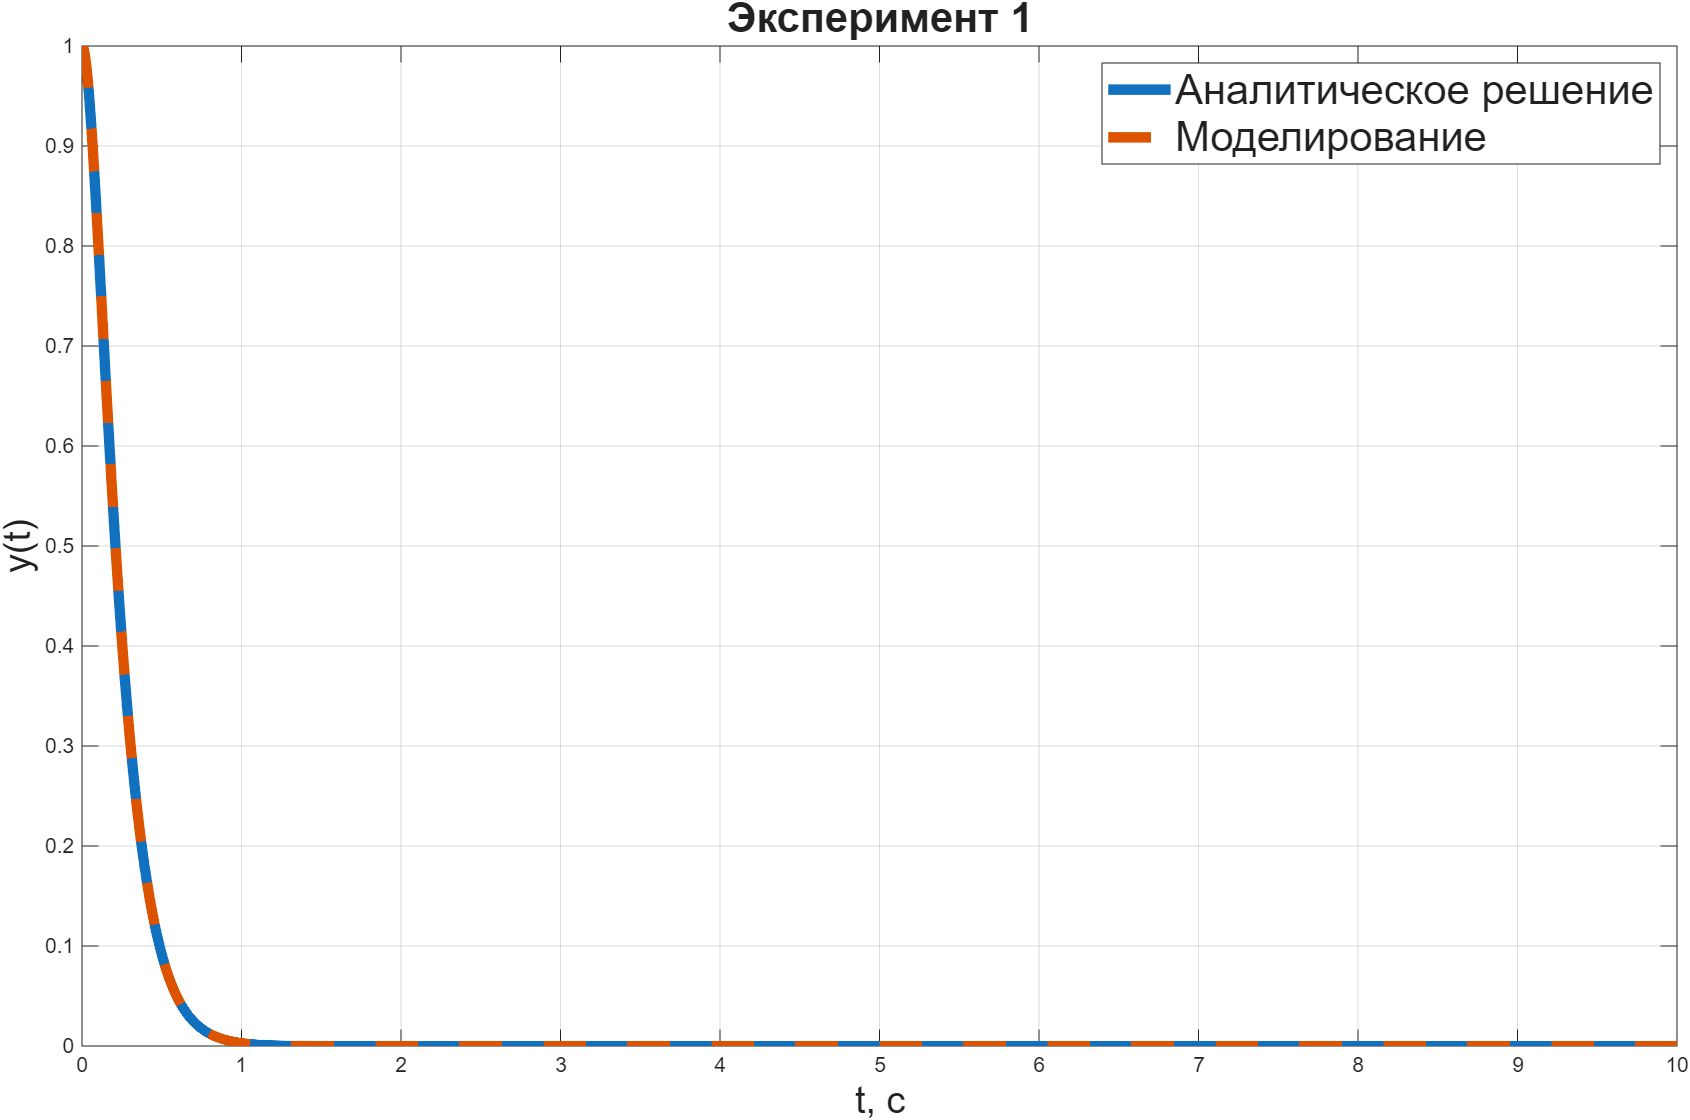
\includegraphics[width=0.8\linewidth]{images/Figure_2_1_1.png}
    \caption{График сравнения для первого эксперимента}
    \label{fig:placeholder}
\end{figure}

\begin{figure}[H]
    \centering
    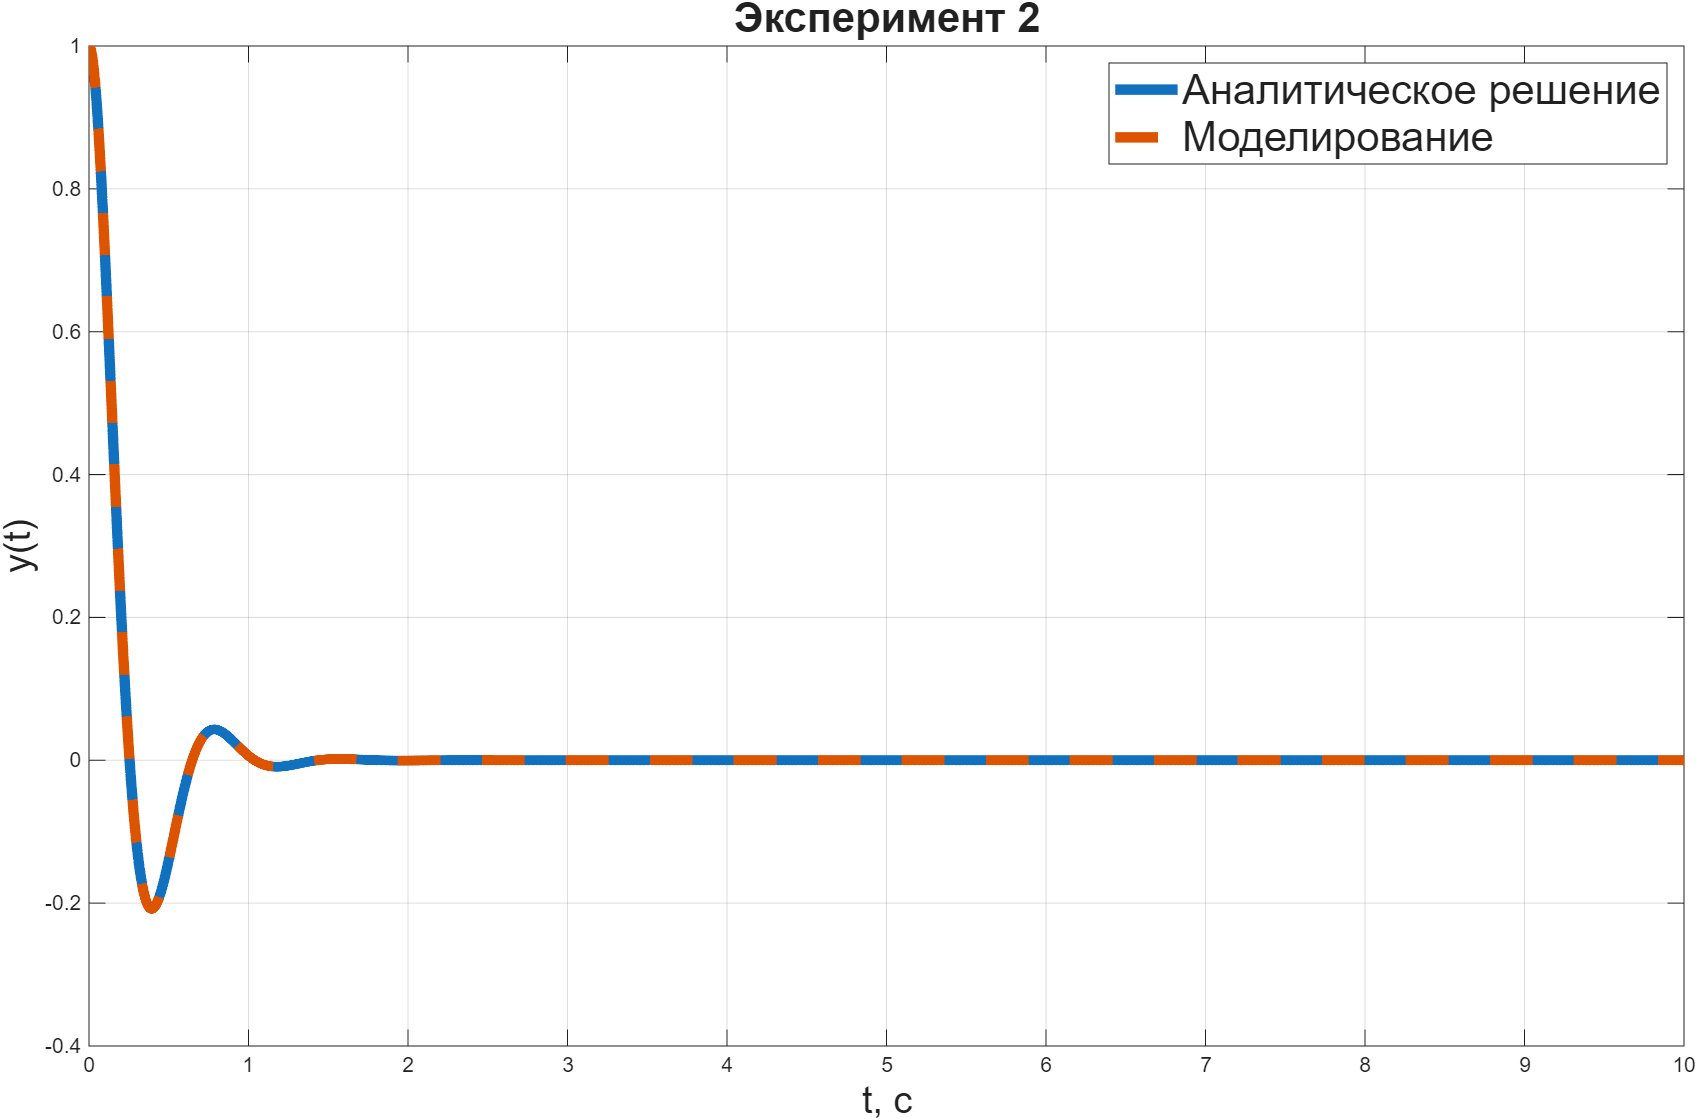
\includegraphics[width=0.8\linewidth]{images/Figure_2_1_2.png}
    \caption{График сравнения для второго эксперимента}
    \label{fig:placeholder}
\end{figure}

\begin{figure}[H]
    \centering
    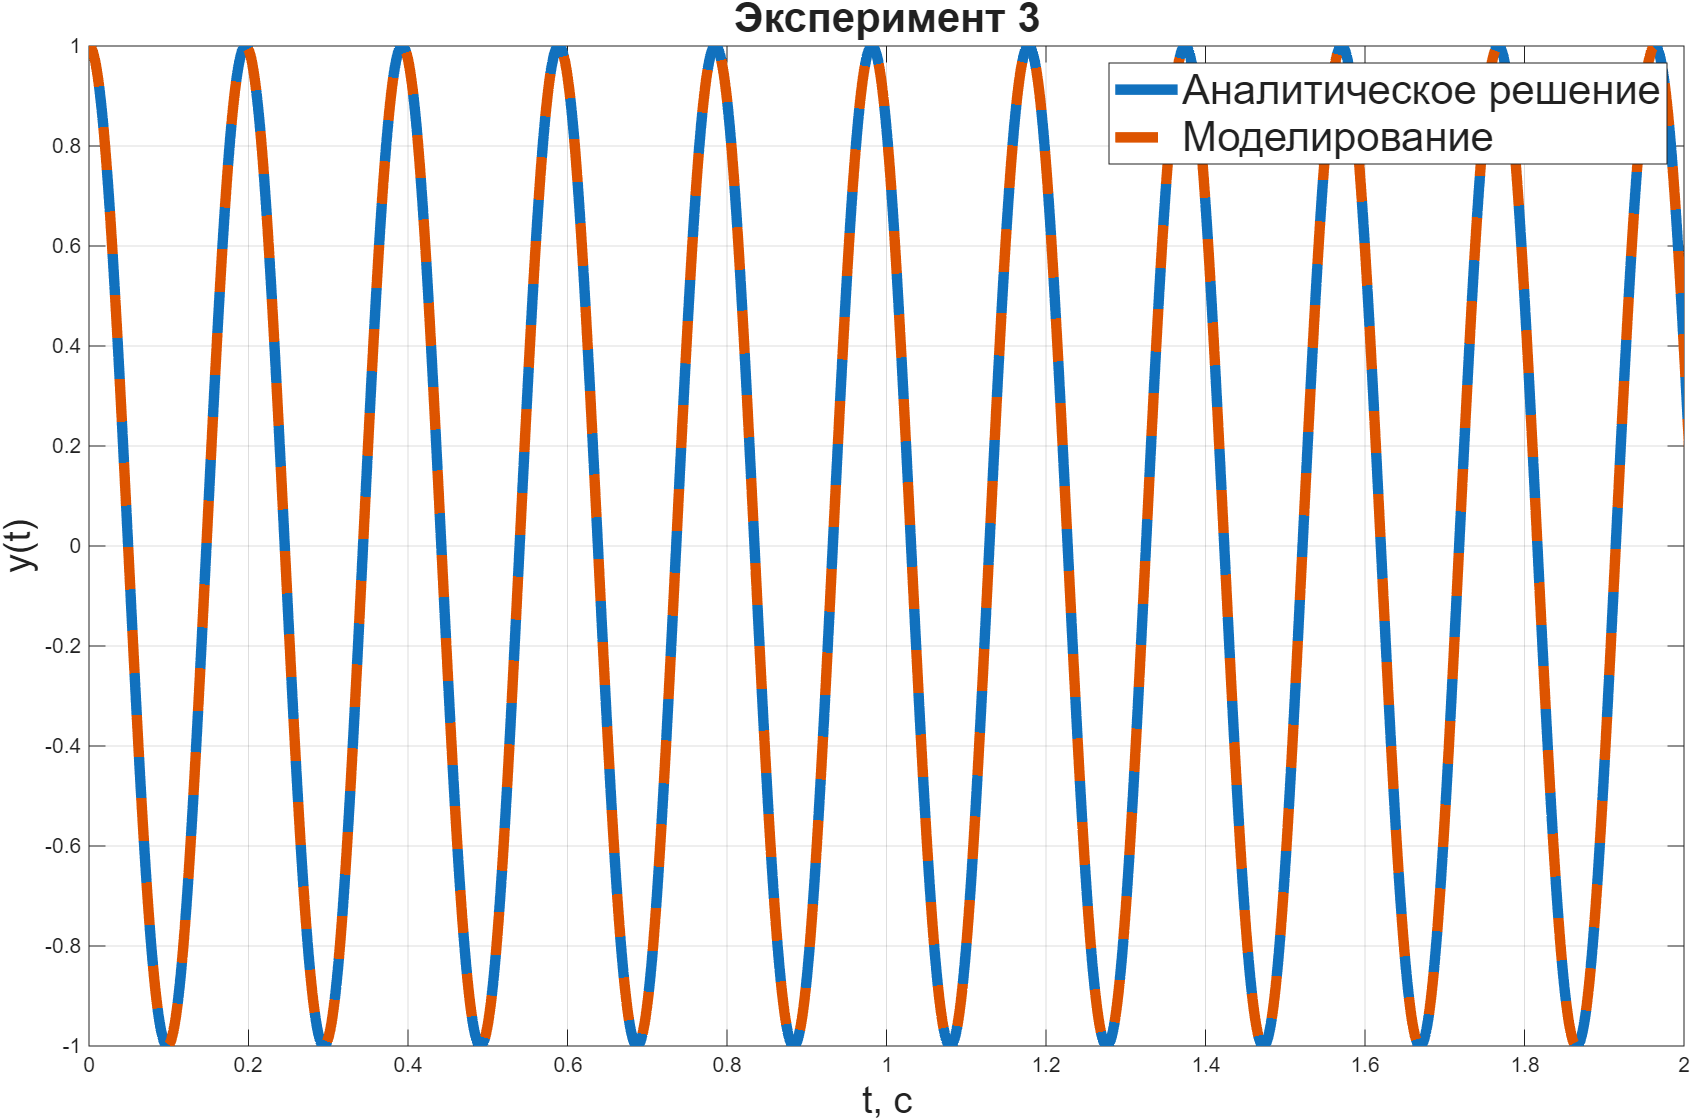
\includegraphics[width=0.8\linewidth]{images/Figure_2_1_3.png}
    \caption{График сравнения для третьего эксперимента}
    \label{fig:placeholder}
\end{figure}

\begin{figure}[H]
    \centering
    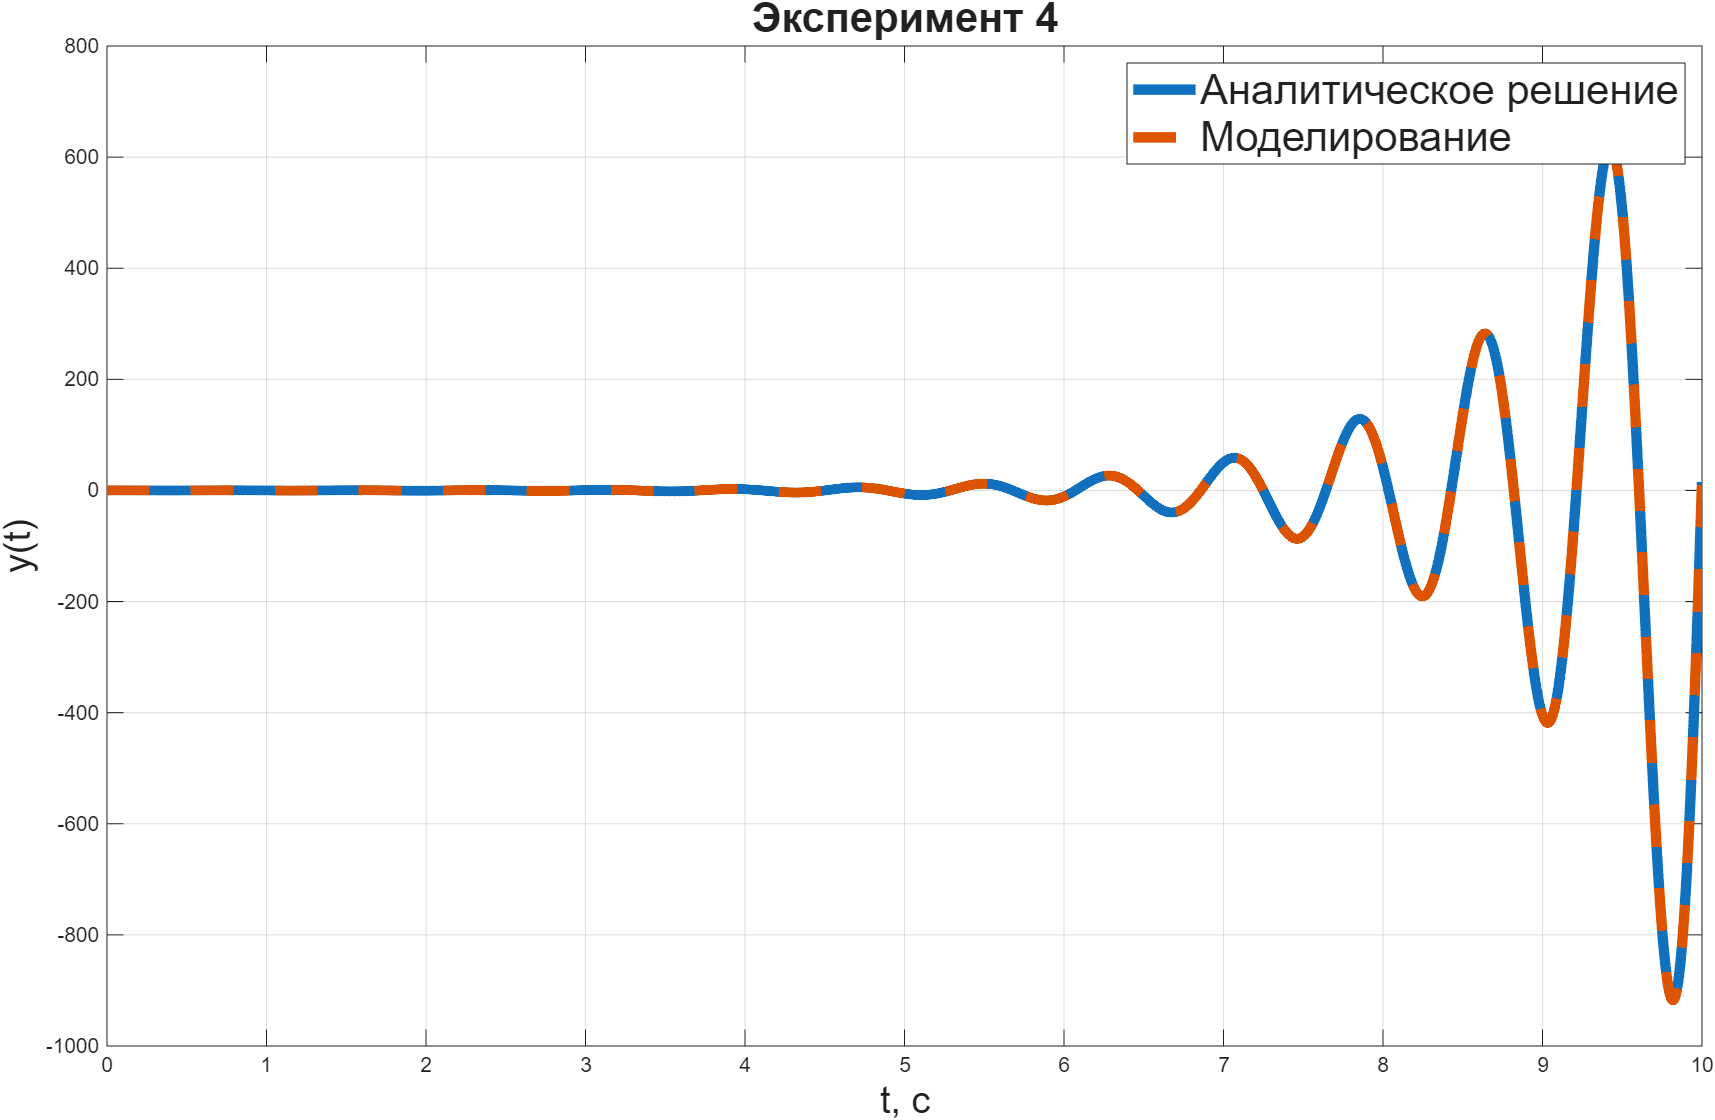
\includegraphics[width=0.8\linewidth]{images/Figure_2_1_4.png}
    \caption{График сравнения для четвертого эксперимента}
    \label{fig:placeholder}
\end{figure}

\begin{figure}[H]
    \centering
    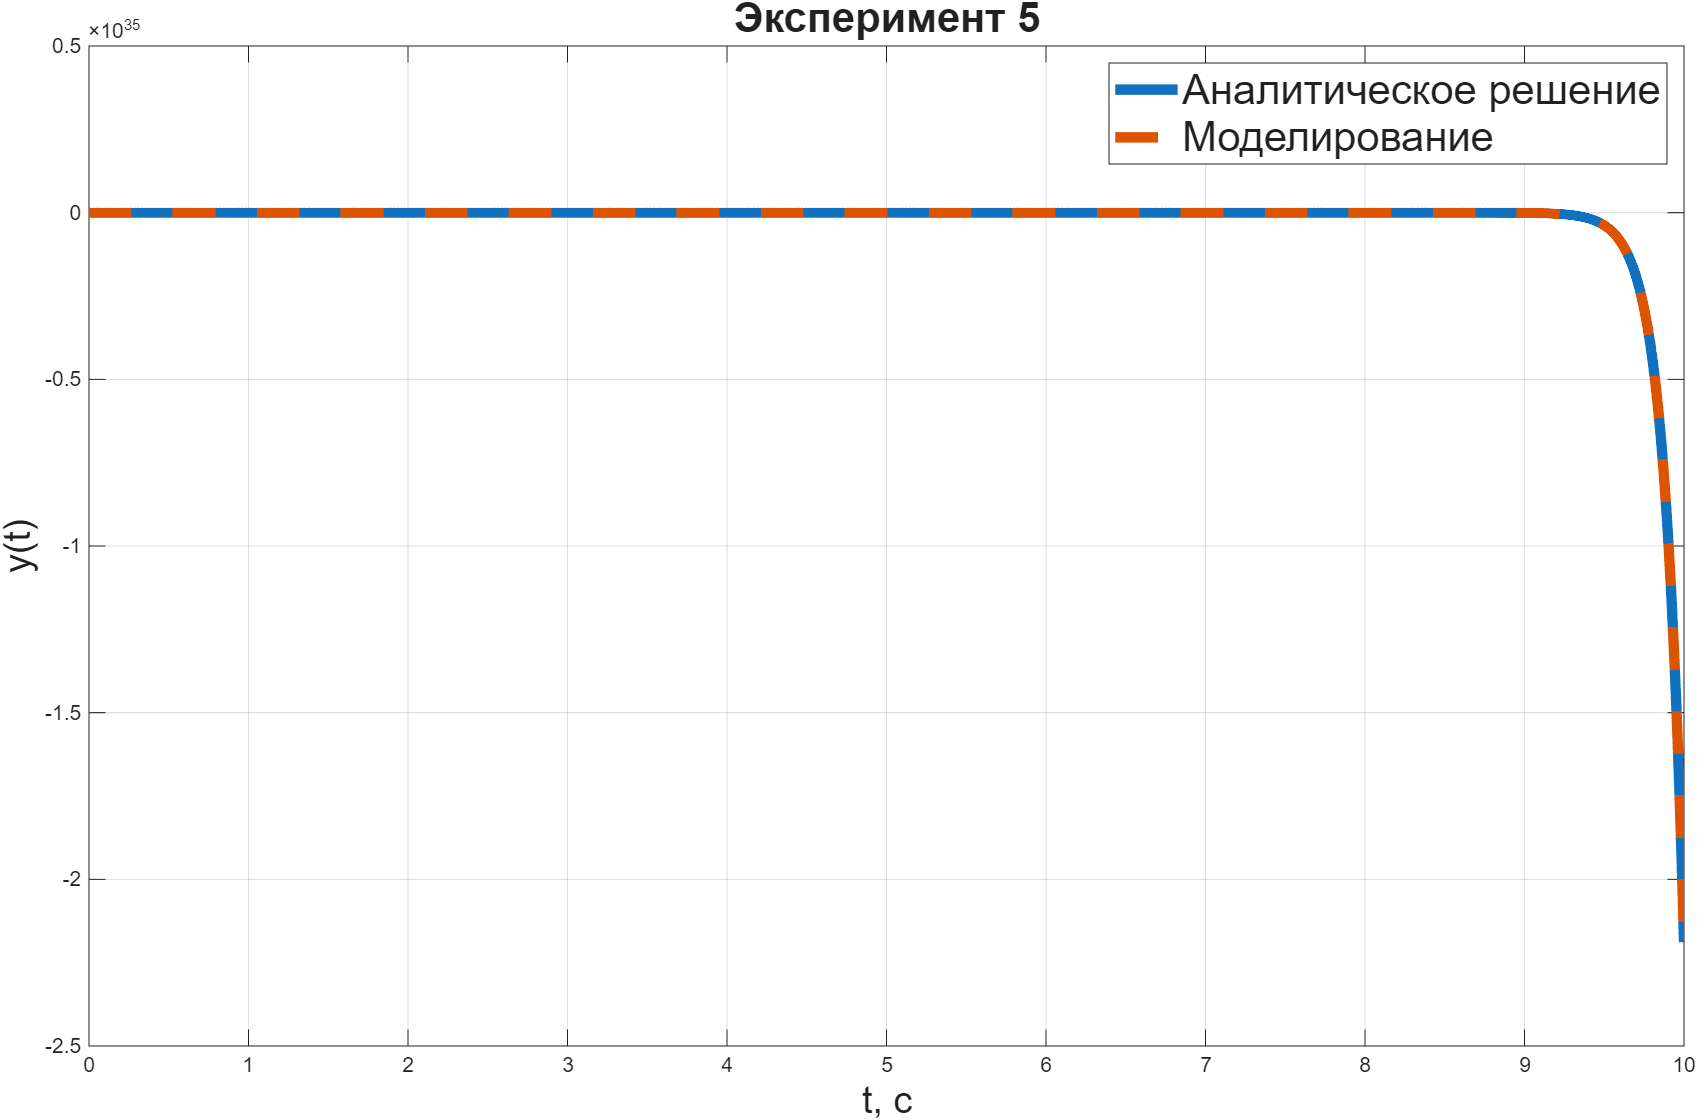
\includegraphics[width=0.8\linewidth]{images/Figure_2_1_5.png}
    \caption{График сравнения для пятого эксперимента}
    \label{fig:placeholder}
\end{figure}

\begin{figure}[H]
    \centering
    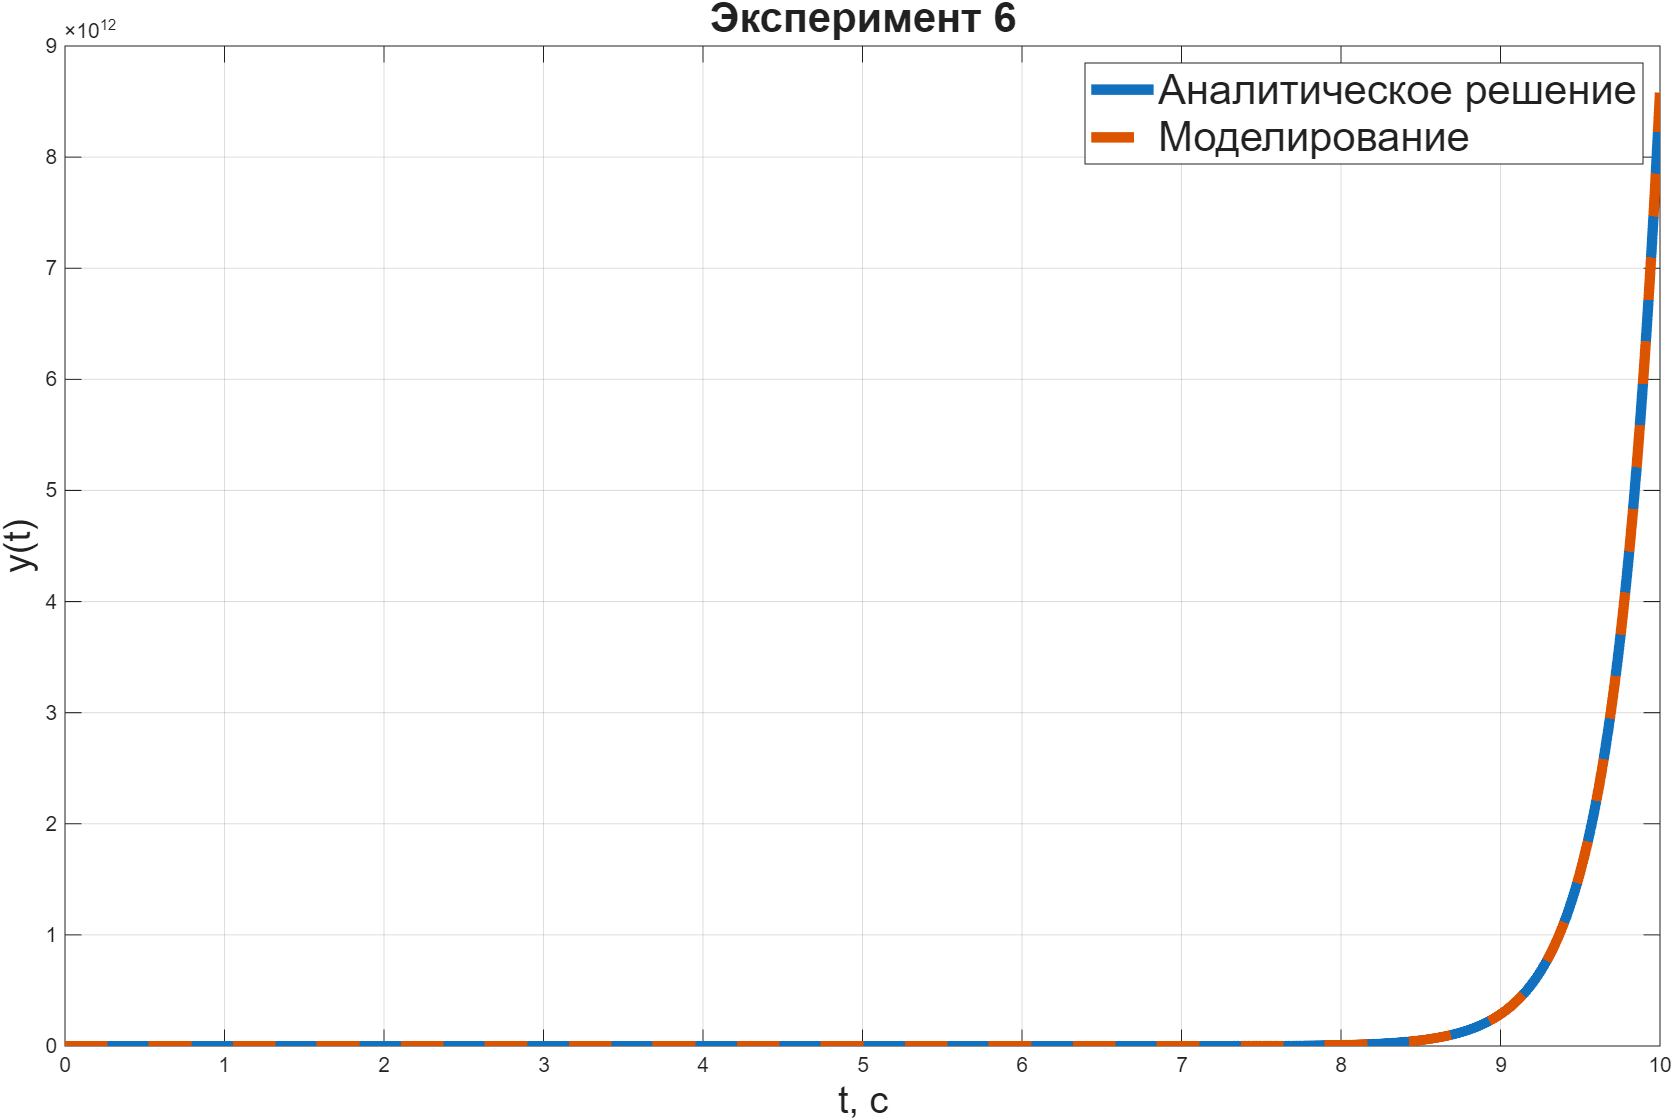
\includegraphics[width=0.8\linewidth]{images/Figure_2_1_6.png}
    \caption{График сравнения для шестого эксперимента}
    \label{fig:placeholder}
\end{figure}

\subsection{Вывод}

Сравнение графиков аналитического решения и моделирования показало их полное совпадение, что подтверждает корректность аналитических вычислений и правильность определения коэффициентов дифференциального уравнения системы. Анализ поведения выходных сигналов позволяет сделать вывод о типе устойчивости системы в зависимости от корней характеристического уравнения: при отрицательных вещественных частях система является устойчивой, при нулевых — находится на границе устойчивости, а при положительных — неустойчива.

\section{Задание 2. Область устойчивости}

\subsection{Исходные данные}

Рассмотрим систему 3-го порядка, заданную структурной схемой:

\begin{figure}[H]
    \centering
    \includegraphics[width=1\linewidth]{images/image_2_2.png}
    \caption{Схема моделирования для Задания 2}
    \label{fig:placeholder}
\end{figure}

\subsection{Листинги аналитических расчетов.}

Система из структурной схемы можно записать в виде:

$$
y=\dfrac{gy-Ky}{p(T_1p+1)(T_2p+1)}
$$

полюса соответствующих придаточных функций совпадут с первым набором корней $\lambda_1$ и $\lambda_2$ при:

$$
\begin{cases}
    T_1\lambda_1+1=0\\
    T_2\lambda_2+1=0
\end{cases}
$$

Подставим $\lambda_1=-8$ и $\lambda_2=-8$:

$$
\begin{cases}
    T_1=\frac{1}{8}\\
    T_2=\frac{1}{8}
\end{cases}
$$

Так как мы рассматриваем свободное движение $g=0$

$$
(p(T_1p+1)(T_2p+1))y=-Ky
$$

$$
y(T_1T_2p^3+(T_1+T_2)p^2+p+K)=0
$$

$$
T_1T_2p^3+(T_1+T_2)p^2+p+K=0
$$

Для полинома третьего порядка
$$
a_3p^3 + a_2p^2 + a_1p + a_0 = 0
$$
условия устойчивости по критерию Гурвица имеют вид:
$$
\begin{cases}
a_3 > 0, \\
a_2 > 0, \\
a_1 > 0, \\
a_0 > 0, \\
a_2a_1 - a_3a_0 > 0.
\end{cases}
$$

В нашем случае:

$$
\begin{cases}
    T_1T_2>0\\
    T_1+T_2>0\\
    1>0\\
    K>0\\
    T_1+T_2-T_1T_2K>0
\end{cases}
$$

$$
0<K(T_1,T_2)<\dfrac{T_1+T_2}{T_1T_2}
$$

$$
\begin{cases}
    0<K(T_1)<8+\dfrac{1}{T_1}\\
    0<K(T_2)<8+\dfrac{1}{T_2}
\end{cases}
$$

\subsection{Графические изображения границ устойчивости.}

\begin{figure}[H]
    \centering
    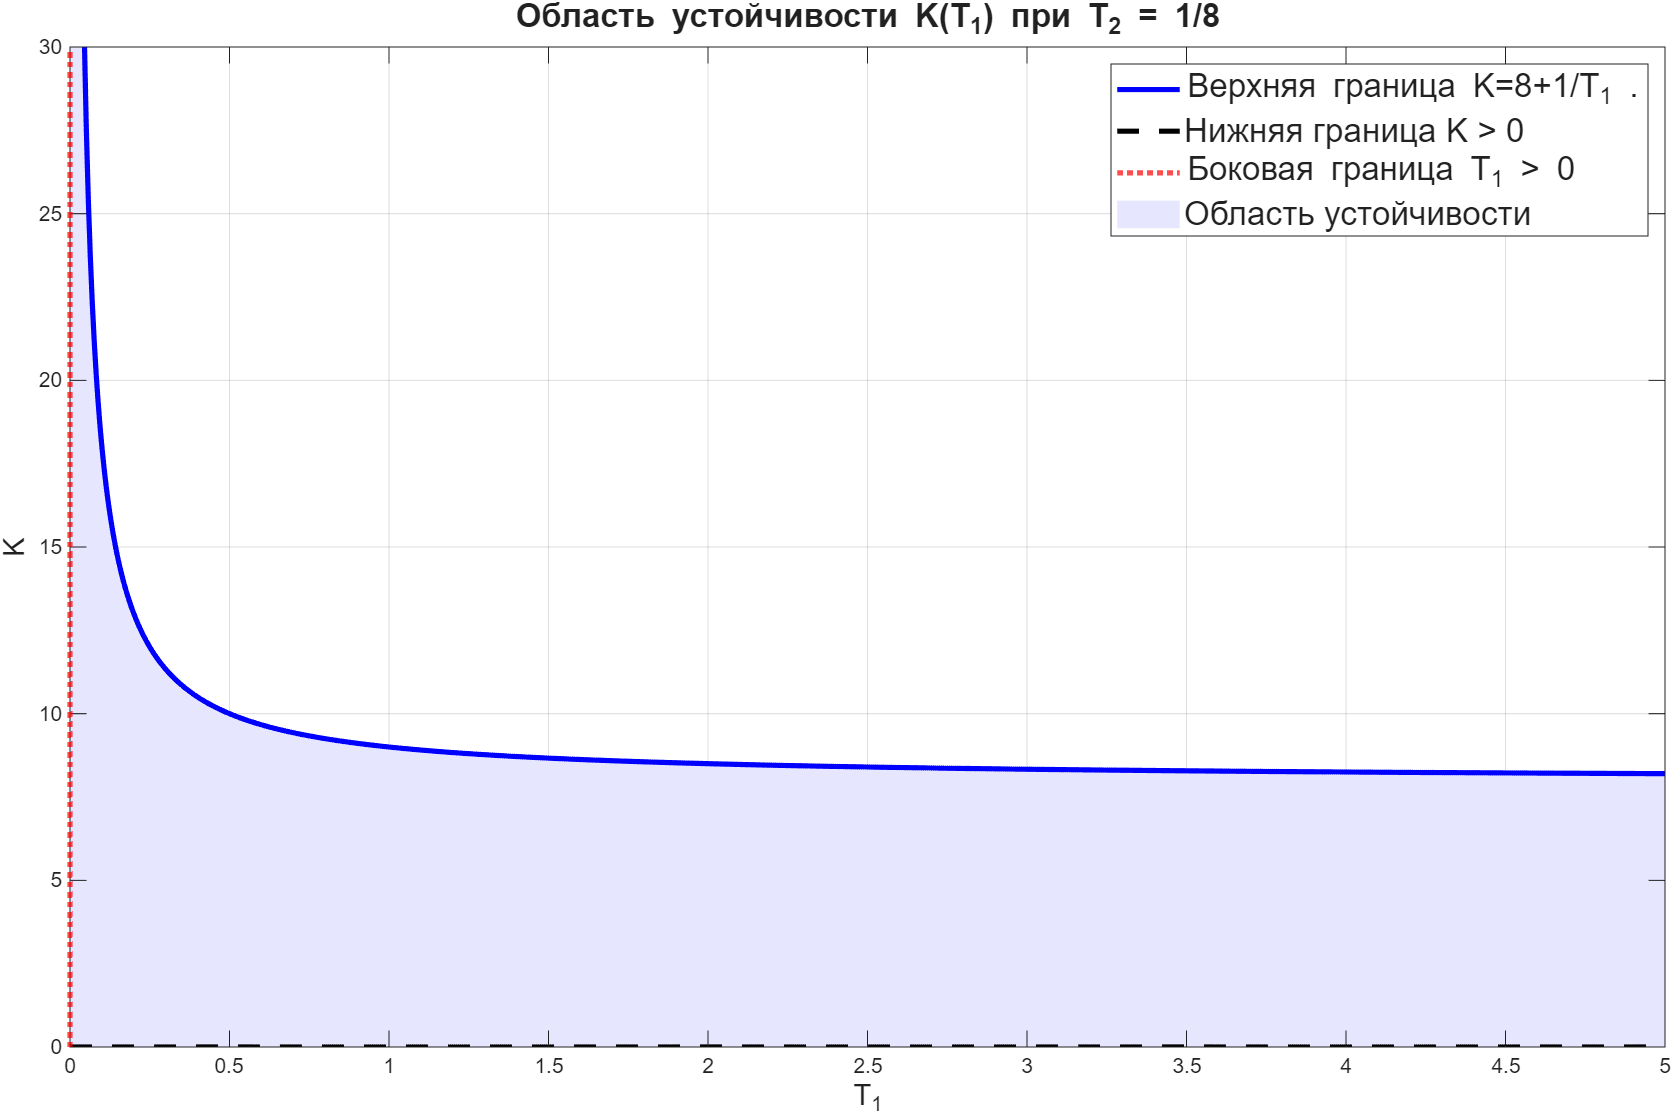
\includegraphics[width=0.8\linewidth]{images/Figure_2_2_1.png}
    \caption{Графическое изображение границы устойчивости для фиксированной $T_2$.}
    \label{fig:placeholder}
\end{figure}

\begin{figure}[H]
    \centering
    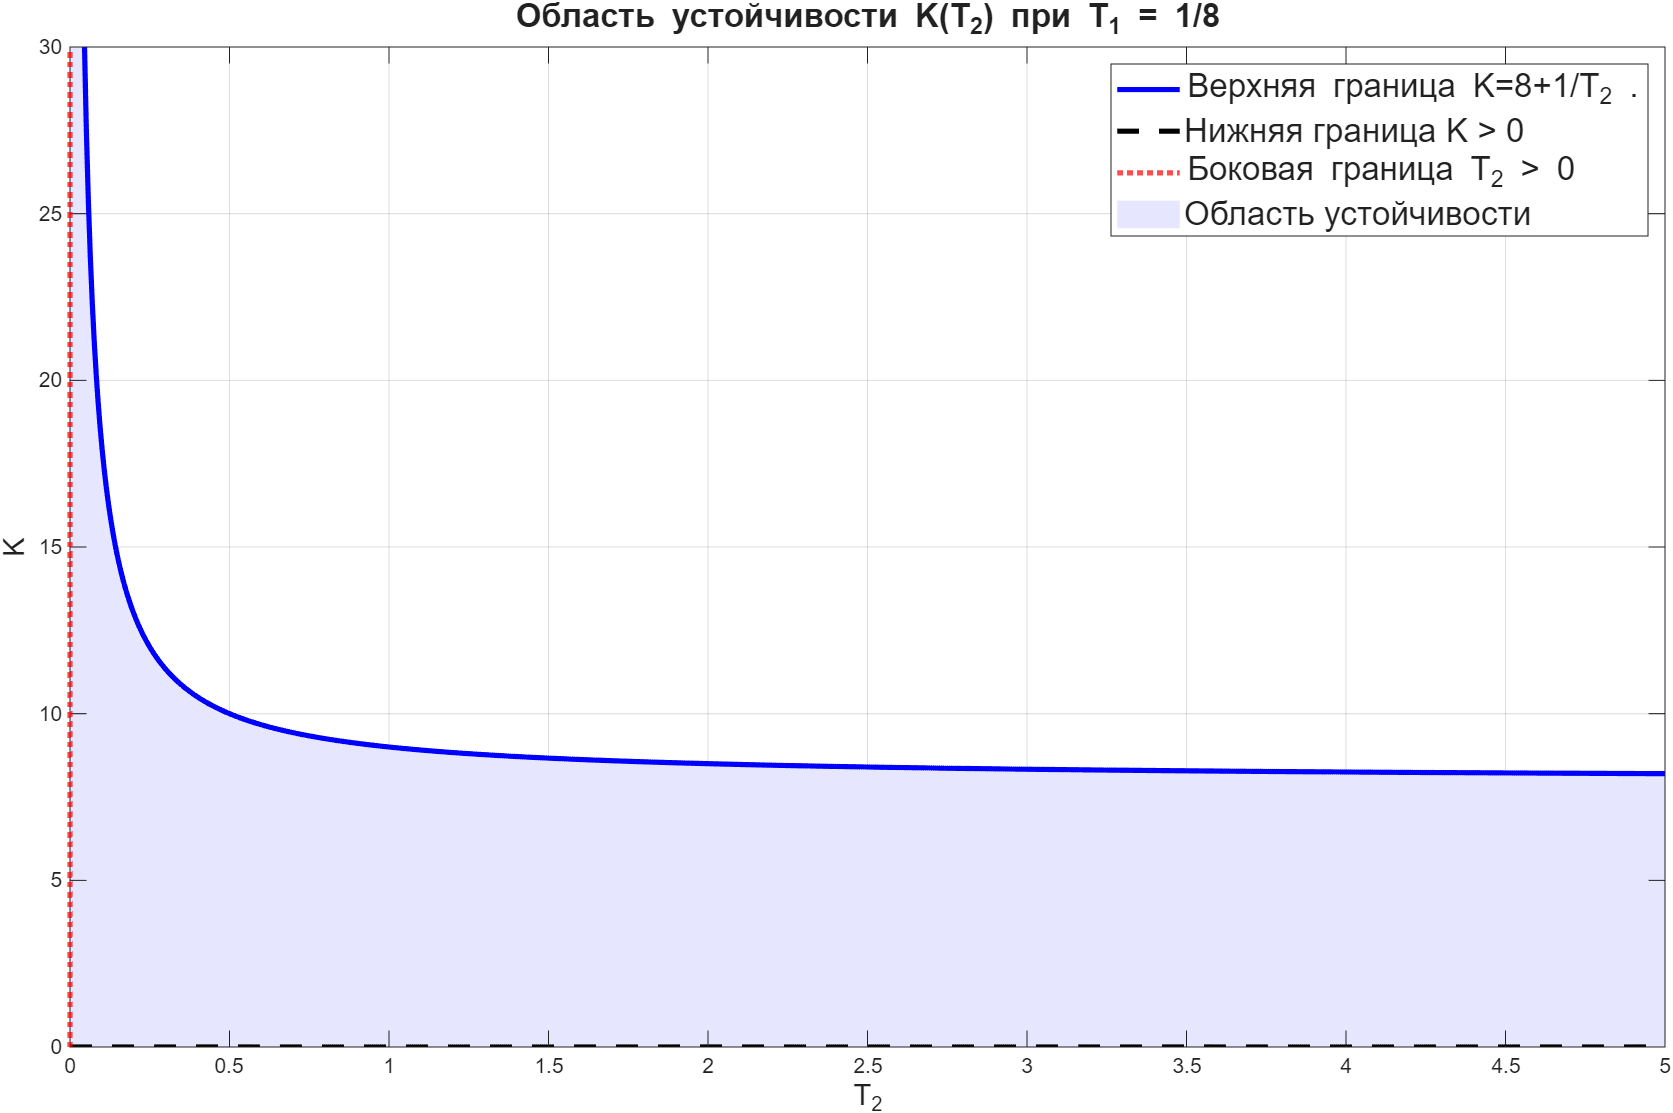
\includegraphics[width=0.8\linewidth]{images/Figure_2_2_2.png}
    \caption{Графическое изображение границы устойчивости для фиксированной $T_1$.}
    \label{fig:placeholder}
\end{figure}

\subsection{Графики выходов $y(t)$ для трех наборов параметров $K$, $T_1$ и $T_2$, соответствующих
различным случаям устойчивости.}

\subsubsection*{Асимптотически устойчивая система}

Пусть $T_1=6$, $T_2=7$, $K=0.1$

$$
K_{\text{гр}}=\dfrac{T_1+T_2}{T_1T_2}=\dfrac{13}{42}
$$

$$
K<K_{\text{гр}}
$$

\begin{figure}[H]
    \centering
    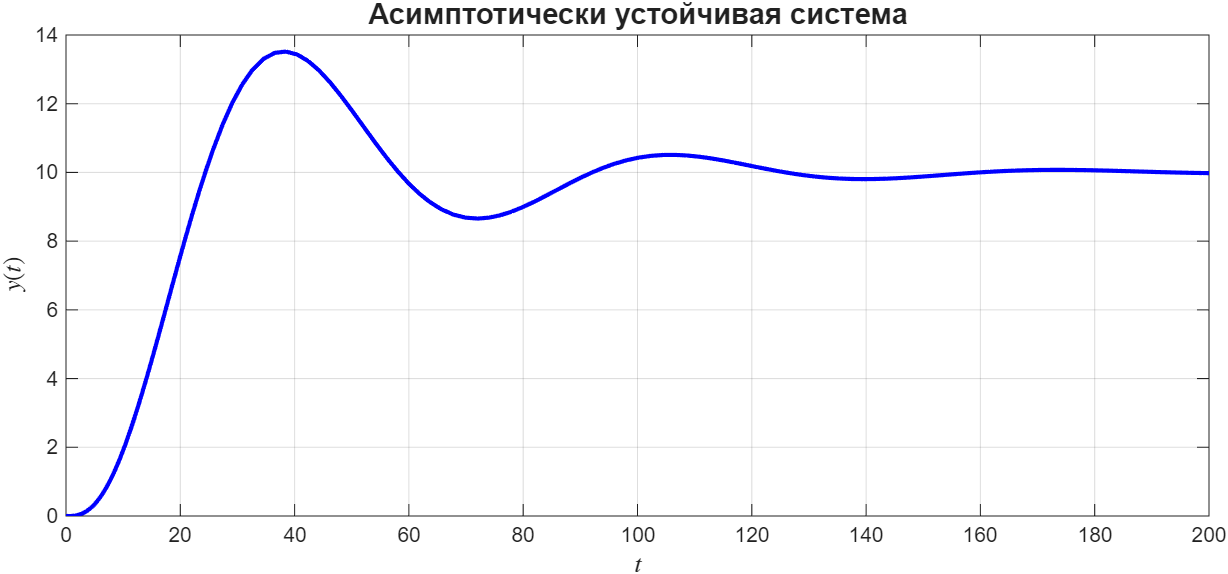
\includegraphics[width=1\linewidth]{images/Figure_2_2_3.png}
    \caption{Асимптотически устойчивая система}
    \label{fig:placeholder}
\end{figure}

\subsubsection*{Система на границе устойчивости}

Пусть $T_1=2$, $T_2=1.2$, $K=\dfrac{4}{3}$

$$
K_{\text{гр}}=\dfrac{T_1+T_2}{T_1T_2}=1.25
$$

$$
K=K_{\text{гр}}
$$

\begin{figure}[H]
    \centering
    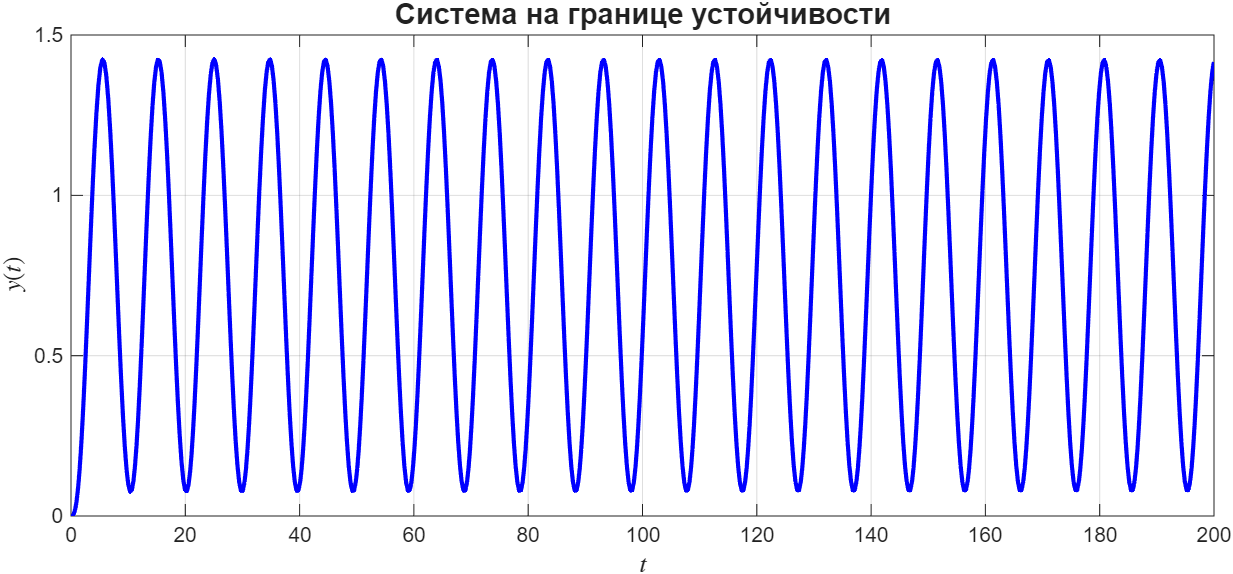
\includegraphics[width=1\linewidth]{images/Figure_2_2_4.png}
    \caption{Система на границе устойчивости}
    \label{fig:placeholder}
\end{figure}

\subsubsection*{Неустойчивая система}

Пусть $T_1=3$, $T_2=5$, $K=2$

$$
K_{\text{гр}}=\dfrac{T_1+T_2}{T_1T_2}=\dfrac{8}{15}
$$

$$
K>K_{\text{гр}}
$$

\begin{figure}[H]
    \centering
    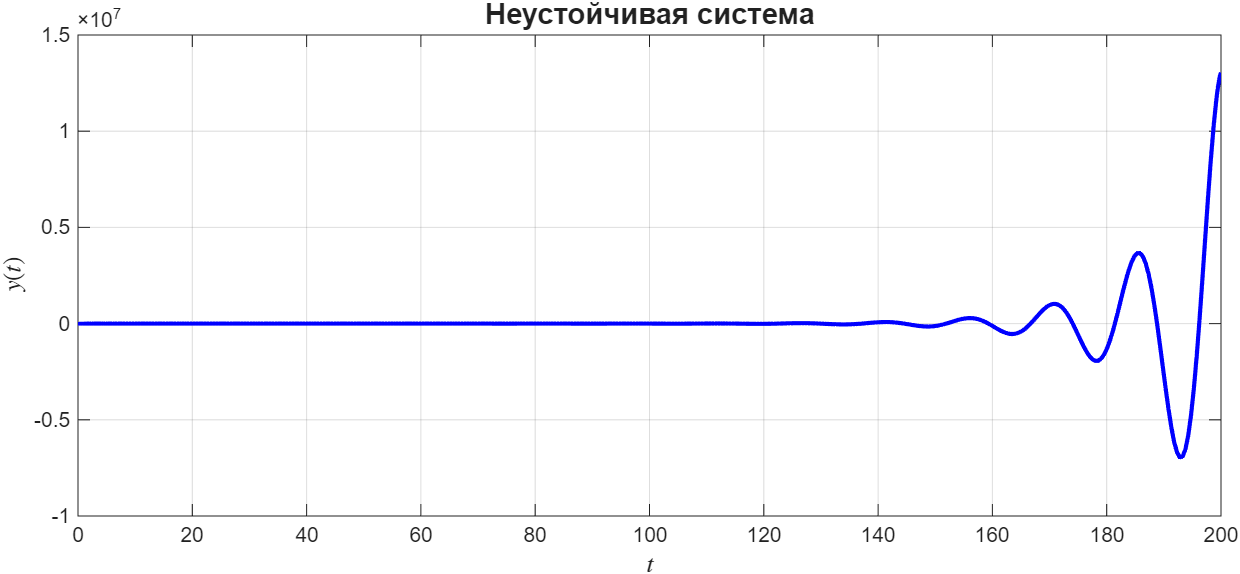
\includegraphics[width=1\linewidth]{images/Figure_2_2_5.png}
    \caption{Неустойчивая система}
    \label{fig:placeholder}
\end{figure}

\subsection{Вывод}

Во втором задании была исследована область устойчивости системы третьего порядка в зависимости от параметров усиления $K$ и постоянных времени $T_1,T_2$. С использованием критерия Гурвица получено аналитическое выражение границы устойчивости, которое определяет допустимые значения параметра $K$ при фиксированных значениях $T_1$ и $T_2$.

Численное моделирование переходных процессов для трёх наборов параметров, соответствующих асимптотически устойчивому, граничному и неустойчивому случаям, подтвердило корректность аналитических выводов. Поведение выходного сигнала $y(t)$ полностью соответствует теоретическим условиям устойчивости.

\section{Задание 3. Автономный генератор}

\subsection{Исходные данные}

Рассмотрим систему:
$$
\begin{cases}
    \dot{x}=Ax\\
    g=Cx
\end{cases}
$$

Нам нужно чтобы $g$ равнялся:

$$g_{\text{ж}}(t)=\cos(9t)+e^{9t}\sin(-t)$$

\subsection{Листинги аналитических расчетов.}

$$
g_{\text{ж}}(t) = \cos(9t) - e^{9t}\sin t.
$$

Первая составляющая $\cos(9t)$ соответствует комплексно-сопряжённой паре собственных значений $\lambda_{1,2} = \pm j9$. Вторая составляющая $e^{9t}\sin t$ соответствует комплексно-сопряжённой паре $\lambda_{3,4} = 9 \pm j$.

$$A = \begin{pmatrix} 
0 & -9 & 0 & 0 \\
9 & 0 & 0 & 0 \\
0 & 0 & 9 & -1 \\
0 & 0 & 1 & 9 
\end{pmatrix}. $$

$$
e^{At}=\begin{bmatrix}
    \cos(9t)&-\sin(9t)&0&0\\
    \sin(9t)&\cos(9t)&0&0\\
    0 & 0 & e^{9t}\cos(t) & e^{9t}-\sin(t) \\
    0 & 0 & e^{9t}\sin(t) & e^{9t}\cos(t) \\
\end{bmatrix}
$$

Запишем вход системы в виде:

$$
g(t)=Ce^{At}x(0)
$$

$$
\begin{aligned}
g(t) &= x_1(0)\bigl[\cos(9t)c_1 + \sin(9t)c_2\bigr] \\
     &\quad + x_2(0)\bigl[-\sin(9t)c_1 + \cos(9t)c_2\bigr] \\
     &\quad +x_3(0)\bigl[ e^{9t}\cos(t)c_3+e^{9t}\sin(t)c_4 \bigr]\\
     &\quad +x_3(0)\bigl[ -e^{9t}\sin(t)c_3+e^{9t}\cos(t)c_4 \bigr]
\end{aligned}
$$

\vspace{0.3cm}

$$
\begin{aligned}
g(t) &=\cos(9t)\bigl[x_1(0)c_1+x_2(0)c_2\bigr]\\ 
     &\quad +\sin(9t)\bigl[x_1(0)c_2-x_2(0)c_1\bigr]\\ 
     &\quad + e^{9t}\cos(t)\bigl[x_3(0)c_3+x_4(0)c_4\bigr]\\
     &\quad + e^{9t}\sin(t)\bigl[x_3(0)c_4-x_4(0)c_3\bigr]\\
\end{aligned}
$$

Подставляем в исходное выражение и получаем:

$$
\begin{cases}
    x_1(0)c_1+x_2(0)c_2=1\\
    x_1(0)c_2-x_2(0)c_1=0\\
    x_3(0)c_3+x_4(0)c_4=0\\
    x_3(0)c_4-x_4(0)c_3=-1
\end{cases}
$$

Пусть:

$$
C=\begin{bmatrix}
    1 & 0 & 0 & 1
\end{bmatrix}
$$

Тогда:

$$
x(0)=\begin{bmatrix}
    1\\
    0\\
    1\\
    0
\end{bmatrix}
$$

\subsection{Значения матриц $A$ и $C$ и начальных условий $x(0)$.}

$$A = \begin{pmatrix} 
0 & -9 & 0 & 0 \\
9 & 0 & 0 & 0 \\
0 & 0 & 9 & -1 \\
0 & 0 & 1 & 9 
\end{pmatrix}. $$

$$
C=\begin{bmatrix}
    1 & 0 & 0 & 1
\end{bmatrix}
$$

$$
x(0)=\begin{bmatrix}
    1\\
    0\\
    1\\
    0
\end{bmatrix}
$$

\subsection{Графики сигналов $g_{\text{ж}}(t)$ и $g(t)$ с их сопоставлением.}

\begin{figure}[H]
    \centering
    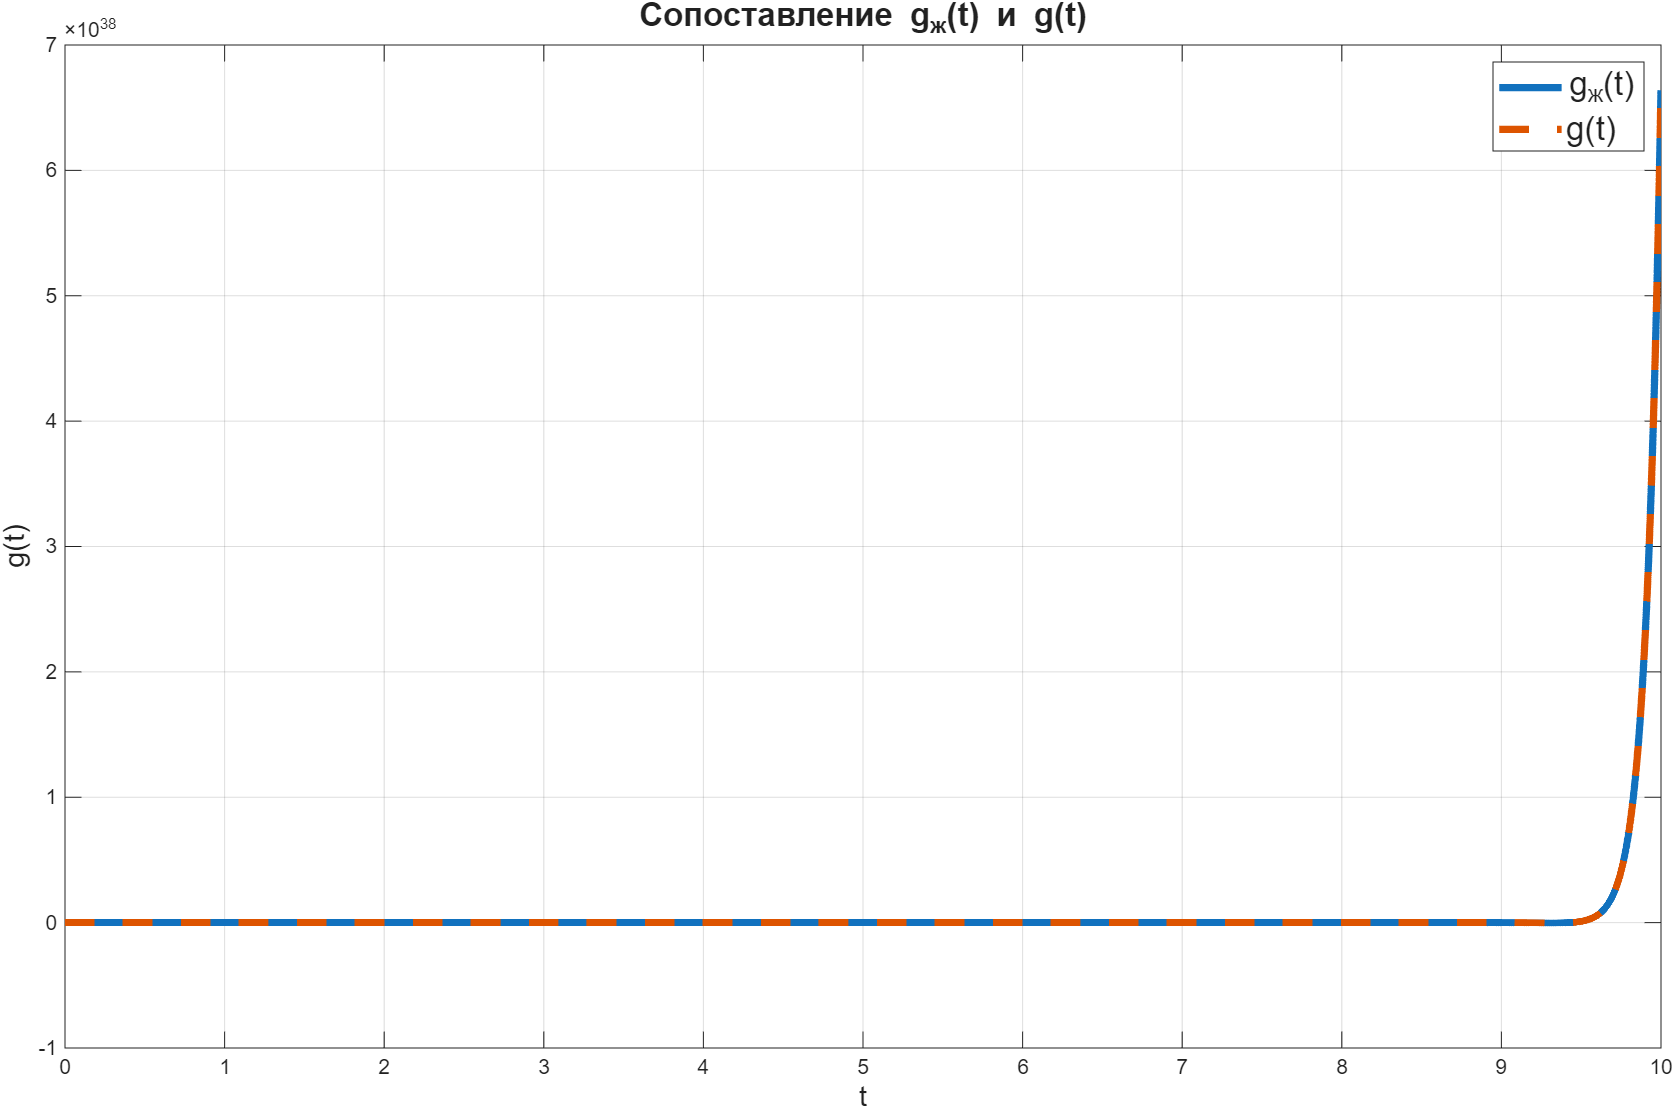
\includegraphics[width=0.8\linewidth]{images/Figure_2_3_1.png}
    \caption{Графики сигналов $g_{\text{ж}}(t)$ и $g(t)$}
    \label{fig:placeholder}
\end{figure}

\subsection{График ошибки $e = g_{\text{ж}}(t) $-$ g(t)$.}

\begin{figure}[H]
    \centering
    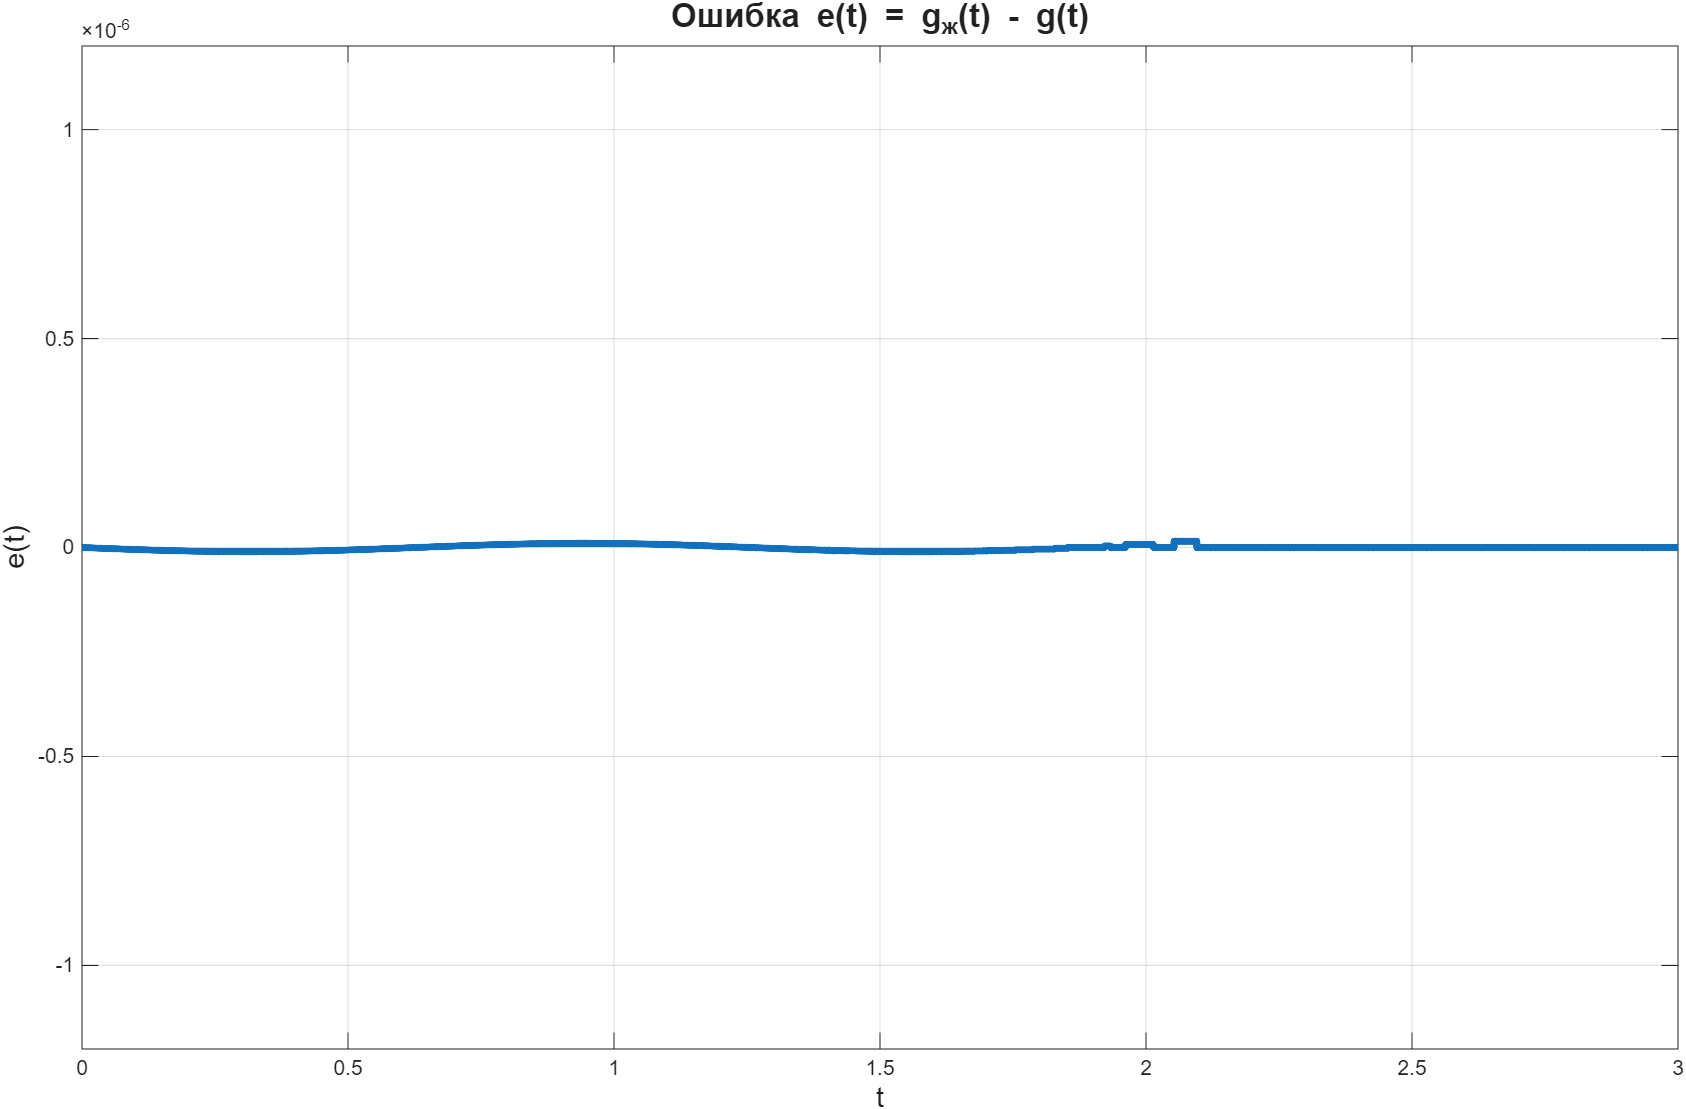
\includegraphics[width=0.8\linewidth]{images/Figure_2_3_2.png}
    \caption{График ошибки $e = g_{\text{ж}}(t)$-$ g(t)$}
    \label{fig:placeholder}
\end{figure}

\section{Вывод}
В ходе выполнения лабораторной работы были исследованы свободное движение, устойчивость линейных систем и синтез автономного генератора

В первом задании была установлена связь между расположением корней характеристического уравнения на комплексной плоскости и устойчивостью системы: при отрицательных вещественных частях система устойчива, при нулевых — находится на границе устойчивости, при положительных — неустойчива.

Во втором задании была исследована область устойчивости системы третьего порядка. С использованием критерия Гурвица определена граница устойчивости, а моделирование подтвердило теоретические выводы о поведении системы в зависимости от выбранных параметров.

В третьем задании синтезирована матрица состояния автономного генератора по заданному выходному сигналу. Результаты моделирования показали точное соответствие между требуемым и полученным сигналами, что подтверждает корректность выбора матриц системы и начальных условий.
\end{document}